\documentclass[10 pt,usenames,dvipsnames, oneside]{article}
\usepackage{../../../modelo-ensino-medio}



\begin{document}

\begin{center}
  \begin{minipage}[l]{3cm}

\includegraphics[width=2cm]{logo}    
\end{minipage}\hfill
\begin{minipage}[r]{.8\textwidth}
 {\Large \scshape Atividade: Estudando o sinal de uma função quadrática com o GeoGebra}  
\end{minipage}
\end{center}
\vspace{.2cm}

\ifdefined\prof
%Habilidades da BNCC
% \begin{objetivos}
% \item 
% \end{objetivos}

%Caixa do Para o Professor
\begin{goals}
%Objetivos específicos
\begin{enumerate}
\item Associar o geogebra ao estudo da variação do sinal de funções quadráticass.
\end{enumerate}

\tcblower

%Orientações e sugestões
Nessa atividade, o objetivo é que o aluno perceba como varia o sinal da função quadrática.
Oriente seus alunos a que reproduzam os itens \titem{a)}, \titem{b)} e \titem{c)} dessa atividade para os casos em que $a>0$ e $\Delta =0, a>0$ e $\Delta <0, a<0$ e $\Delta>0, a<0$ e $\Delta=0, a<0$ e $\Delta<0$.
\end{goals}

\bigskip
\begin{center}
{\large \scshape Atividade}
\end{center}
\fi

Vamos fazer uma construção usando o GeoGebra. Siga os seguintes passos:

1-	Abra a janela gráfica e escreva $y=a(x-p)^2+q$ no campo de entrada e tecle ENTER;

\begin{figure}[H]
\centering
\noindent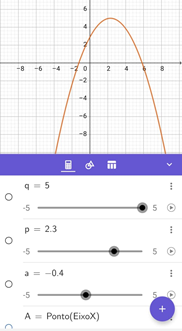
\includegraphics[width=150bp]{inequacao4}
\end{figure}

Observe que o GeoGebra denominou por $f$ à função que associa $x$ e $y$ por meio da lei algébrica $y=a(x-p)^2+q$ e gerou, automaticamente, três controles deslizantes para os valores de $a$, $p$ e $q$, variando de $-5$ a $5$. Movimente os controles deslizantes e verifique o que ocorre com a função. Quais os significados geométricos, na parábola, dos parâmetros $a$, $p$ e $q$?

\begin{figure}[H]
\centering
\noindent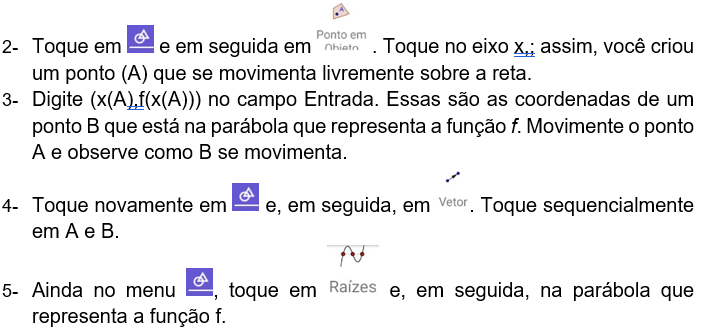
\includegraphics[width=400bp]{icones2}
\end{figure}
Agora vamos explorar um pouco a sua construção?

\begin{enumerate}
\item{} Ajuste o controle deslizante $a$ para um valor maior que zero. Como está a concavidade da função $f$?

\item {} Mantenha o controle deslizante $a$ fixo com o valor usado no item \titem{a)}. Arraste o ponto $A$ para o canto mais esquerdo do eixo $x$ e ajuste os controles $p$ e $q$ de forma que tenhamos duas raízes para a função $f$. Qual o sinal do discriminante $\Delta$?

\item{}	
Movimente lentamente o ponto $A$ no sentido positivo do eixo $x$. O que você observa sobre o vetor $\overrightarrow{AB}$? Descreva a posição desse vetor de acordo com as raízes da função $f$.
\end{enumerate}

\ifdefined\prof
\begin{solucao}

\begin{enumerate}
\item Para cima.
\item Positivo.
\item O vetor $AB$ alterna o seu sentido de cima para baixo exatamente quando o ponto $A$ passa pelo primeiro zero da função quadrática e depois de baixo para cima quando passa pelo segundo zero da função quadrática.
\end{enumerate}

\end{solucao}
\fi

\end{document}